\chapter{$D^0 \to \mu^+\mu^-$ Branching Fraction Measurement}

\section{Analysis overview}

TODO

\section{Triggers and datasets}

\subsection{Data samples}

The events used for this analysis are collected from proton-proton collisions at the LHC at a center of mass of 13.6 TeV. Specifically, we use data from the CMS detector during the years 2022 and 2023. The CMS collaboration marks specific run ranges as good runs and groups them into datasets marked with letters. The data we use is denoted as 2022C, 2022D, 2022E, 2022F, 2022G, 2023C, and 2023D. 

There are two triggers used for the analysis:
\begin{enumerate}
    \item The \texttt{HLT\_DoubleMu4\_3\_LowMass} trigger is used to collect $D^{*\pm} \to D^0 \pi^\pm, D^0 \to \mu^+ \mu^-$ signal events by triggering on the dimuon final product. During the collection of the data samples of the analysis, the trigger was virtually unchanged and unprescaled, making it convenient to use for signal collection.
    \item The \texttt{HLT\_ZeroBias} trigger was used to collect $D^{*\pm} \to D^0 \pi^\pm, D^0 \to \pi^+ \pi^-$ normalization events. Unlike the signal trigger, this trigger does not filter for a specific signature. However, the expected branching fraction of $D^{*\pm} \to D^0 \pi^\pm, D^0 \to \pi^+ \pi^-$ is large enough to generate a sufficient number of desired events. During the collection of the data samples of the analysis, the trigger was virtually unchanged and was prescaled at the HLT and L1 triggers on the order of 1e6. 
\end{enumerate}

The events collected by these two triggers and grouped into two datasets, ZeroBias and Parking DoubleMuonLowMass, respectively. We use the NanoAOD file format, designed by CMS to contain ntuples of per-event information and used for most analysis at CMS. Specifically, we use the NanoAODv12 recipe which is processed from MiniAOD. In this processing, we apply the muon data certification to ensure high quality muon objects. 

\subsection{Backgrounds}

A key component of the analysis is the accurate modeling of background, specifically because of how small the anticpated limit of the signal strength is. There are two main types of backgrounds to consider: 
\begin{enumerate}
    \item Combinatorial backgrounds: backgrounds which are characterized by noise from random combinations of particles produced in secondary particle collisions. 
    \item Peaking backgrounds: backgrounds which are characterized by a peaking structure near the signal region.
\end{enumerate}

\subsubsection{Combinatorial Backgrounds}

TODO: INSERT Combinatorial background section

\subsubsection{Peaking Backgrounds}

Unlike combinatorial backgrounds, peaking backgrounds must be carefully studied to ensure that the background peak in the signal region is not modeled as signal. These peaking backgrounds occur most commonly from detector misreconstruction. For example, pions can be misreconstructed as muons, resulting in some $D^0 \to \pi^+ \pi^-$ events being reconstructed as $D^0 \to \mu^+ \mu^-$ events, causing a peaking background near the signal region. Specifically, we know that pions and kaons are the only 2 particles which are (1) common decay products of the $D^0$ and (2) are relatively frequently misreconstructed as muons\footnote{See section TODO: add section for pion and kaon fake rates}. Therefore, the candidates for peaking background are two body hadronic decays of the $D^0$ meson and non-$D^{*\pm} \to D^0 \pi^\pm$ decays. 

For each of the peaking backgrounds, we check their $\Delta m$ and dimuon mass against the $\Delta m$ and dimuon mass of the signal. While the non-$D^{*\pm} \to D^0 \pi^\pm$ decays exhibit a dimuon mass distribution which is virtually identical to the signal, their $\Delta m$ contribution is expected to be combinatorial so they do no overlap with the signal's signature. The dominate two body hadronic decays of the $D^0$ meson therefore are the only contributions to peaking background and are listed below.
\begin{enumerate}
    \item $D^0 \to \pi^+ \pi^-$
    \item $D^0 \to K^\pm \pi^\mp$
    \item $D^0 \to K^+ K^-$
    \item $D^0 \to \pi^\pm \mu^mp$
\end{enumerate}
For each of these, we use \texttt{TGenPhaseSpace} to simulate the effects of the misreconstructed on the peaking background distributions in both $\Delta m$ and the invariant dimuon mass and compare them to the signal distribution. As can be seen in figure \ref{fig:reconstructed_D0_comparison}, every decay except $D^0 \to \pi^+ \pi^-$ gives a distribution which is distinct from the signal distribution in either $\Delta m$ or the dimuon invariant mass. Therefore, the only peaking distribution which we must model and account for is $D^0 \to \pi^+ \pi^-$. 

\begin{figure}[htp]
    \begin{center}
      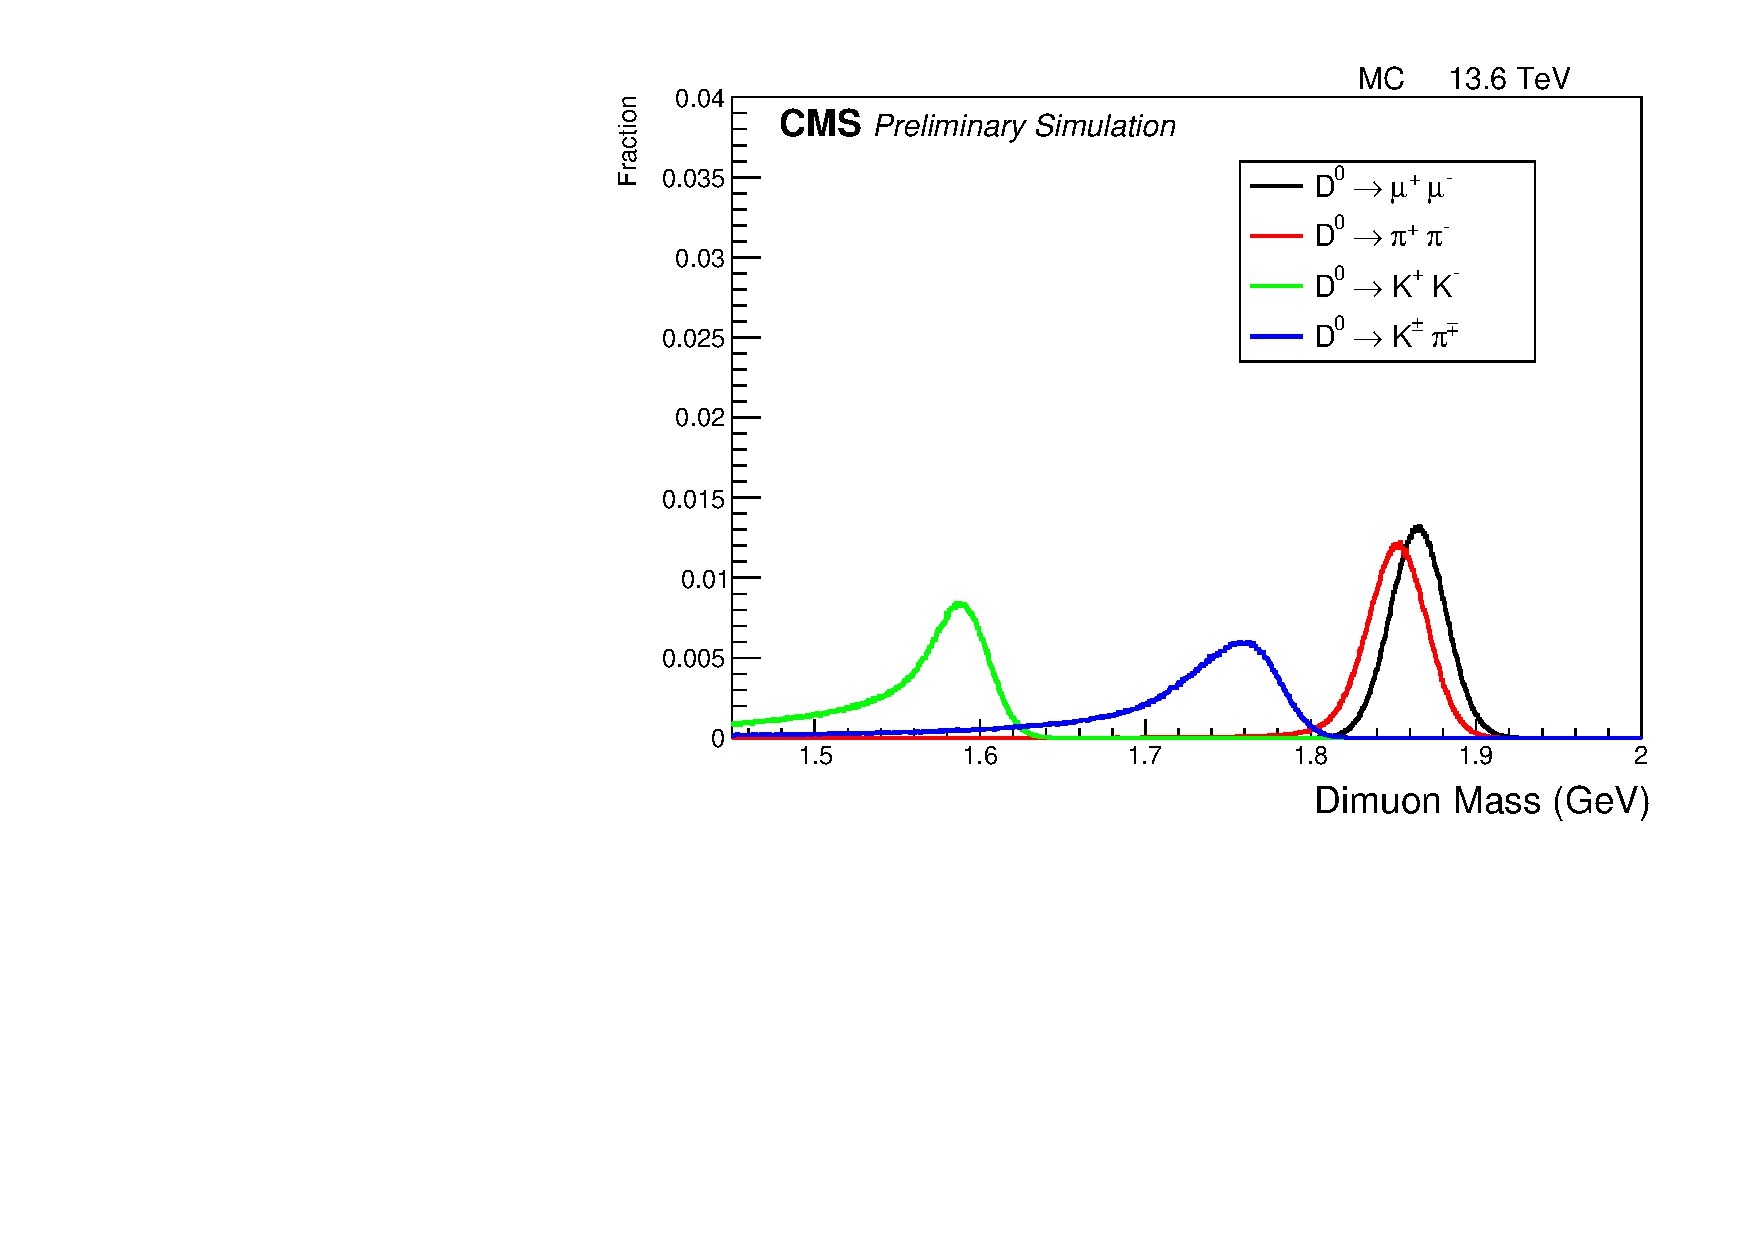
\includegraphics[width=0.45\textwidth]{figures/chapter4/reconstructed_D0_mass.pdf}
      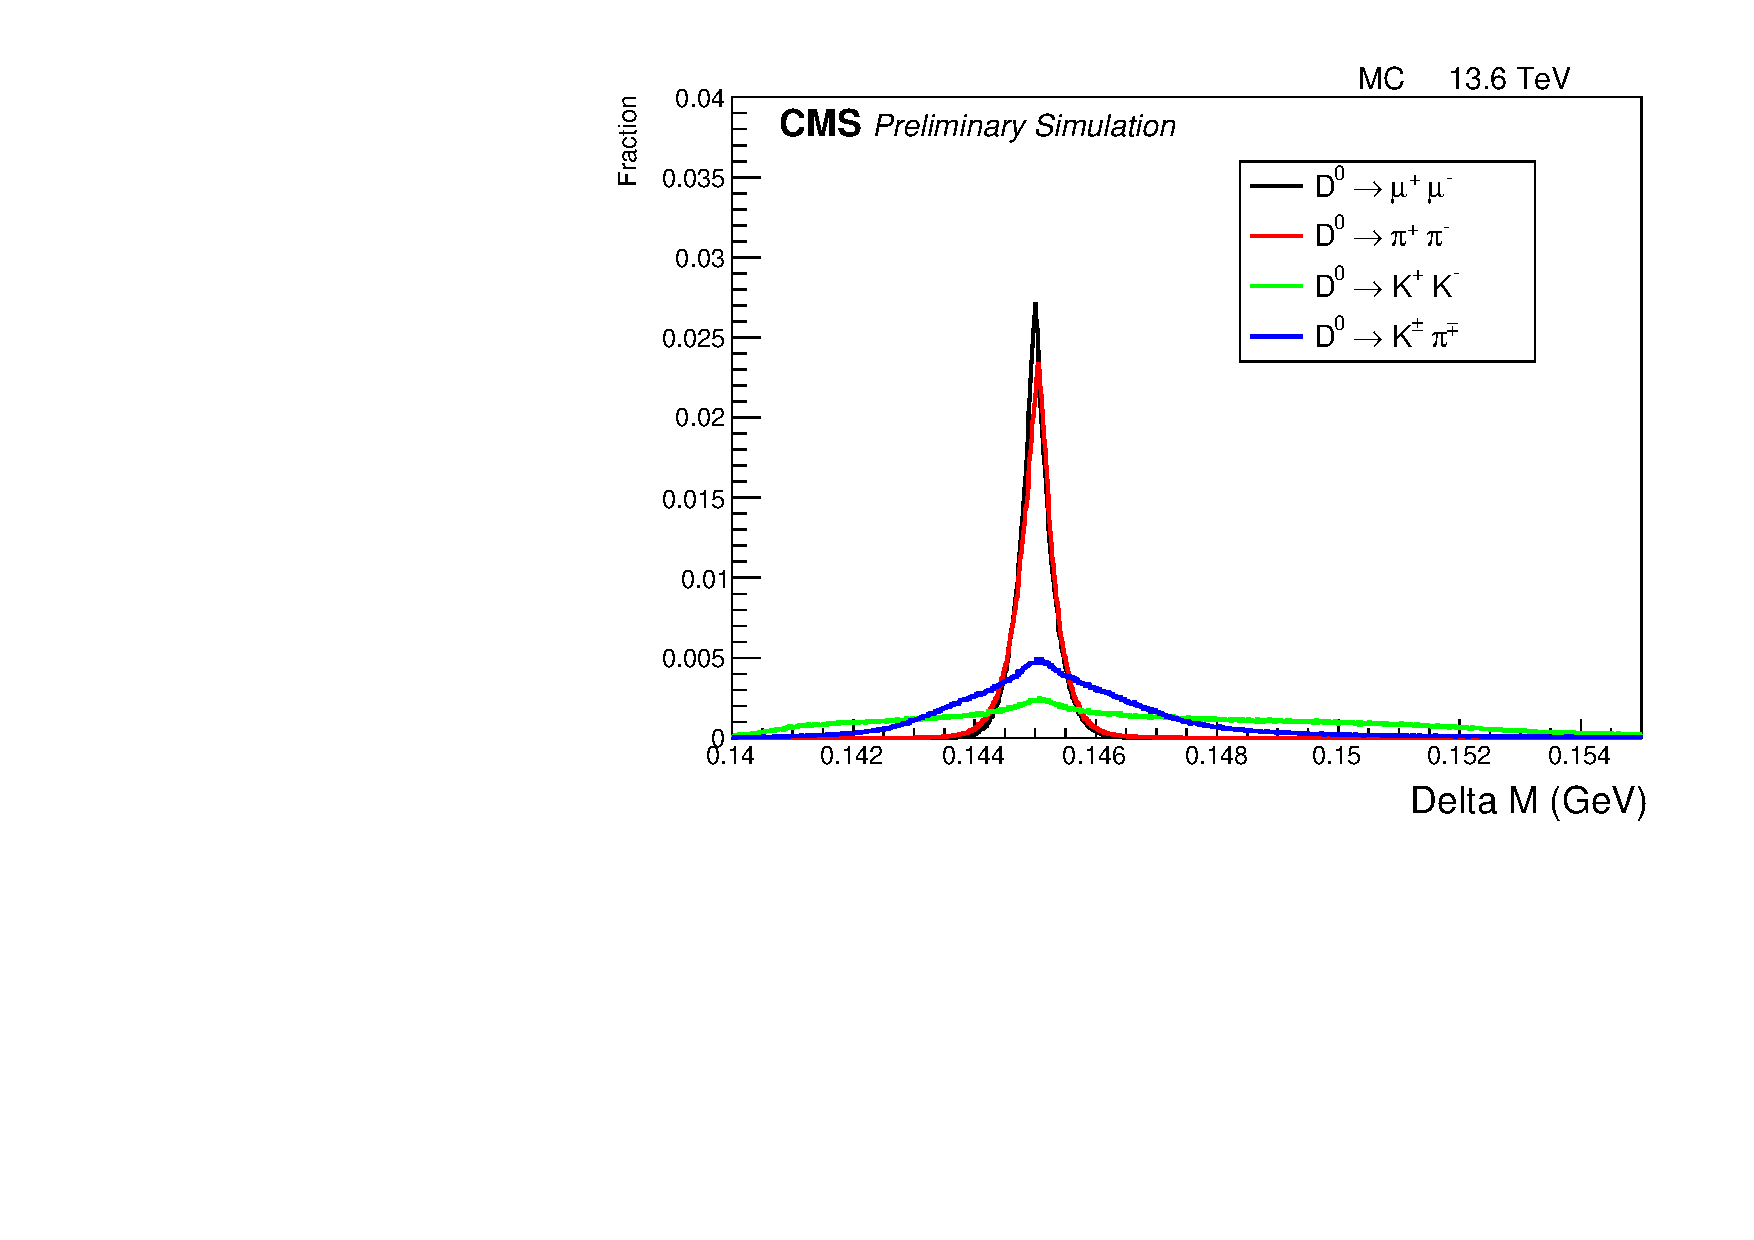
\includegraphics[width=0.45\textwidth]{figures/chapter4/reconstructed_delta_m.pdf}\\
    \end{center}
    \caption{
      Comparison of normalized frequencies for various peaking background $D^0 \to \mu^+ \mu^-$ decays against the signal decay.
      Right: Reconstructed $\Delta m$ distribution.
      Left: Reconstructed dimuon mass distribution, where decay products are forced to take the muon mass using \texttt{TGenPhaseSpace}, even for non-dimuon final states.
    }
    \label{fig:reconstructed_D0_comparison}
  \end{figure}
  
  


\subsection{Monte Carlo samples}

TODO

\section{Selections and efficiency}

Once we've attained the data and monte carlo samples needed for this analysis, we filter through them using event selections, carefully tracking the \textit{acceptance} and \textit{efficiency} for each selection\footnote{We define \textit{acceptance} as TODO and \textit{efficiency} as TODO}. The selection process can be broken down into three main stages:
\begin{enumerate}
    \item The \textit{preselection} stage provides the selections which are tied to trigger requirements, reconstruction requirements, and dataset size limitations.
    \item The \textit{baseline selection} stage primarily is used to reject background samples while keeping the efficiency high, the sidebands of the signal region large, and the signal shape unperturned. 
    \item The \textit{multivariate analysis (MVA) selection} stage uses ML-methods to optimize the background rejection.
\end{enumerate}

\subsection{Preselection}
\label{subsec:preselection}

The preselection is used to create reconstructed event candidates which pass the triggers discussed in section TODO. To stay consistent between signal and normalization events, we keep a similar preselection process for both $D^{*\pm} \to D^0 \pi^\pm, D^0 \to \mu^+ \mu^-$ and $D^{*\pm} \to D^0 \pi^\pm, D^0 \to \pi^+ \pi^-$ events.

In order to properly reconstruct the $D^{*\pm} \to D^0 \pi^\pm, D^0 \to \mu^+ \mu^-$ and $D^{*\pm} \to D^0 \pi^\pm, D^0 \to \pi^+ \pi^-$ events, we first must reconstruct their decay products: the muons and pion. Pions are reconstructed from charged tracks found in the tracker. These track are reconstructed using particle flow (PF) algorithms\footnote{The primary goal of these algorithms is to reconstruct individual particles using the data read out from the detector itself. This is made especially difficult because of the high lumonisties of run3 resulting in a large amount of \textit{pileup}, a phenomenon that occurs due to multiple proton-proton collisions happening within a very short time frame resulting in multiple collisons per event. }, meaning the pions used in the analysis are labeled as PF candidates. Muons are reconstructed primarily using detector read out from the muon chambers. We use the well established CMS reconstruction algorithms \texttt{TrackerMuon} and \texttt{GlobaleMuon} as well as use the collaboration's \texttt{LooseMuonID} for muon identification. To reduce background noise and increase detector resolution, we also cut at $p_T>4$ GeV and require a \texttt{highPurity} inner track in the tracker for both pions and muons.

Once we have the muon and/or pion candidates for the $D^0$ decay, we use vertex reconstruction to reconstruct the full decay candidate. A \textit{vertex} is the location in 3D space where a process occured and the \textit{primary vertex} is the location of the interaction of the quarks of the two colliding protons, which in our case produce the $D^{*\pm}$. Due to the short mean lifetime of the $D^{*\pm}$ ($ 6.9 \pm 1.9 \times 10^{-21} \; s$) \cite{ref:pdg2024}, we can label the $D^{*\pm} \to D^0 \pi^\pm$ vertex using the primary vertex. The kinematic vertex reconstruction begins by identifying the dimuon or dipion decay candidates (i.e two pions or two muons which came from the same decay). The two 4-momentum vectors of these two candidates is added together to get a dimuon or dipion 4-momentum vector. We call this dimuon/dipion system a $D^0$ candidate. Using the $D^0$ candidate 4-momentum vector, we calculate the transverse momentum of $D^0$ candidate and extrapolate it to its intersection with the beamline. Then, in order to determine which primary vertex\footnote{There are often many primary vertices in one event due to pileup} the $D^{*\pm} \to D^0 \pi^\pm$ decay came from, we calculate the 3D distance between each primary vertex candidate and the extrapolated intersection point, known as the \textit{3D-impact parameter}, and find the primary vertex which minimizes this parameter. Lastly, since the decay at the primary vertex is $D^{*\pm} \to D^0 \pi^\pm$, we check if there exists a soft pion which came from the selected primary vertex. This kinematic vertex reconstruction is then used to gather reconstructed signal and normalization events as well as refit the $D^0$ candidates to a common vertex using a kinematic vertex fitting tool (TODO: insert citation), generating \textit{refitted} candidates. The events which pass this reconstruction are thus the events that pass the preselection. 

\begin{figure}[htbp]
    \centering
    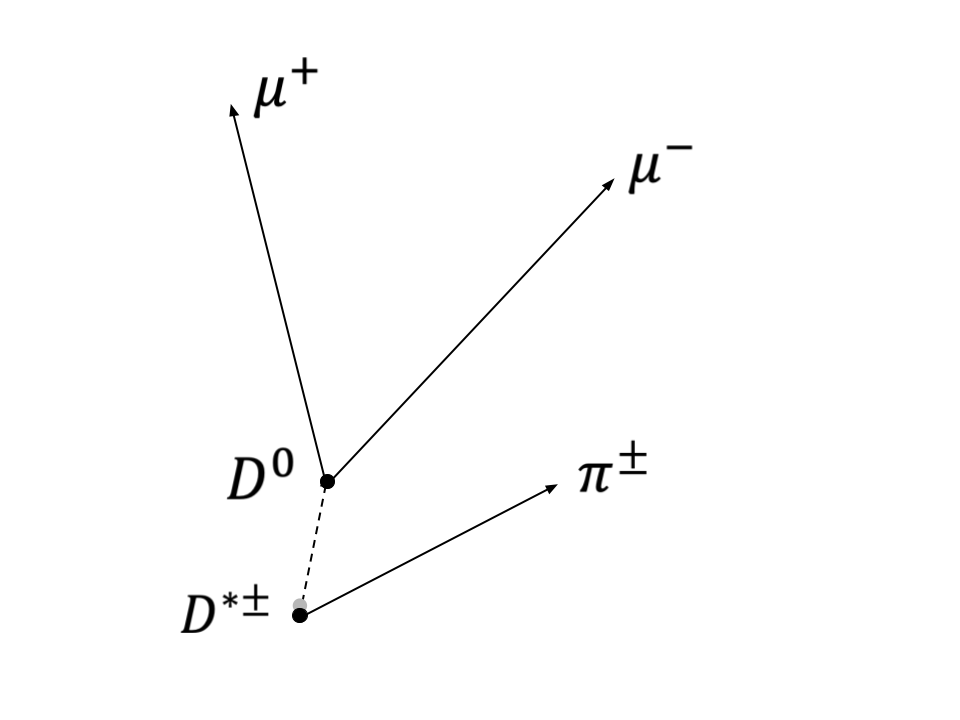
\includegraphics[width=0.8\textwidth]{figures/chapter4/vertex_reconstruction.png}
    \caption{An example of the $D^{*\pm} \to D^0 \pi^\pm, D^0 \to \mu^+ \mu^-$ vertex}
    \label{fig:vertex_reconstruction}
\end{figure}

\subsection{Baseline selection}

Using the reconstruction described in section \ref{subsec:preselection}, we are able to extract several kinematic variables from $D^{*\pm} \to D^0 \pi^\pm$ candidates outputted by the preselection. These variables are used in the baseline selection as well as in other parts of the analysis. They are defined here as follows:
\begin{enumerate}
    \item Reconstructed $D^0$ mass: the mass calculated from from the addition of the two 4-momentum vectors of the $D^0$'s product candidates (either dimuon or dipion). 
    \item Refitted $D^0$ mass: the mass calculated from from the addition of the two 4-momentum vectors of the $D^0$'s product candidates (either dimuon or dipion) once they have been refitted using the kinematic vertex fitting. 
    \item Reconstructed $\Delta m$: the mass difference between the reconstructed $D^{*\pm}$ candidates and the reconstructed $D^0$ candidates. 
    \item Refitted $\Delta m$: the mass difference between the $D^{*\pm}$ and the $D^0$ candidates once they have been refitted using the kinematic vertex fitting.
    \item $\delta_{3D}$: the 3D impact parameter as defined in section \ref{subsec:preselection})
    \item $\delta_{3D}/\sigma\left(\delta_{3D}\right)$: the significance of the 3D impact parameter. This is calculated by taking the value of the 3D impact parameter and dividing it by the square root of the expected variance of the parameter. 
    \item $l_{3D}$: the 3D distance between the vertex of the $D^{*\pm} \to D^0 \pi^\pm$ decay (primary vertex) and the vertex of the $D^0 \to l l$ decay. This can also be called the $\textit{flight length}$ of the $D^0$ meson. 
    \item $l_{3D}/\sigma\left(l_{3D}\right)$: the significance of the 3D distance between the vertex of the $D^{*\pm} \to D^0 \pi^\pm$ decay (primary vertex) and the vertex of the $D^0 \to l l$ decay. Calculated by taking the value of the distance and dividing it by the square root of the expected variance of the distance. 
    \item $l_{xy}$: the distance in the $xy$ plane (perpendicular to the beam line) between the vertex of the $D^{*\pm} \to D^0 \pi^\pm$ decay (primary vertex) and the vertex of the $D^0 \to l l$ decay.  This can also be called the $\textit{transverse flight length}$ of the $D^0$ meson. 
    \item $l_{xy}/\sigma\left(l_{xy}\right)$: the significance of the distance in the $xy$ plane between the vertex of the $D^{*\pm} \to D^0 \pi^\pm$ decay (primary vertex) and the vertex of the $D^0 \to l l$ decay. Calculated by taking the value of the distance and dividing it by the square root of the expected variance of the distance. 
    \item $\alpha_{3D}$ : the angle between the $D^0$ momentum and flight direction. 
    \item $D^0$ vertex probability: the probability given by the $\chi^2$ fit which reconstructs the $D^0$ vertex 
    \item $D^*$ vertex probability: the probability given by the $\chi^2$ fit which reconstructs the $D^*$ vertex
\end{enumerate}
Note that, unless otherwise stated, the refitted variables are used over the reconstructed ones. 

Using these variables, we impart a baseline selection on the preselected events. The goal of the baseline selection is to reject much of the background while keeping the signal efficiency high and not perturbing the signal shape. To achieve this, we select a $D^0$ reconstructed mass in the range of TODO INSERT RANGE, $D^0$ refitted mass in the range of TODO: INSERT RANGE, reconstructed $\Delta m$ in the range of TODO: INSERT RANGE, and refitted $\Delta m$ in the range TODO: INSERT RANGE. As seen in figure TODO: INSERt FIGURE, these ranges are picked such that there are large sidebands on the signal, keeping signal efficiency high as shown in table: TODO INSERT TABLE.

The other set of baseline selections are on the vertices themselves. We require the $D^*$ vertex probability to be greater that $0.1$ and the $D^0$ vertex probability to be greater than $0.01$. This is done such that there is some confidence in the vertex reconstruction and such that we can match the double muon trigger requirement of $0.005$. To gain further confidence in the vertex reconstruction, we limit $\alpha_{3D} < 0.1$ radians and the flight length significance to be greater than 3. Lastly, to keep the normalization channel (which is gathered from a ZeroBias trigger) under the same selection as the signal channel (which is gather from a HLT\_DoubleMuon trigger), we require the event in the normalization channel to have fired the \texttt{HLT\_DoubleMu4\_3\_LowMass} trigger. Note, this does not mean than the specific decay we reconstruct fired the trigger, in fact usually some other event has fired the trigger. 

TODO: insert figure of variable plots

TODO: insert table of efficiencies


\subsection{Multivariate Analysis}

The preselection and baseline selections optimize signal efficiency, but not overall analysis sensitivity. In order to optimize the analysis sensitivity, we train a classifier using a decision tree model driven multivariate analysis (MVA). This single classifying parameter can then be used as a selection parameter named $\text{MVA}_D$ and the cut can be tuned to optimize analysis sensitivity.

The decision tree model used is based on the XGBoost (Extreme Gradient Boosting) library, which builds a forest of regression trees trained sequentially to minimize a regularized objective function. Each tree in the sequence focuses on correcting the erros of the previous tree and the scores from the trees are combined to get a final prediction on the classifiction of the event from the forest. Each tree is constructed using a greedy algorithm that selects splits based on gain, with regularization terms penalizing model complexity to prevent overfitting. The loss function is binary logistic loss, which is optimized using boosting under second-order gradient information with an evaluation metric based on the area under the receiver-operating characteristic (ROC) curve, known as AUC in the literature. Each tree has a maximum depth of 3 and is trained using a learning rate of $\eta = 0.1$. An additional regularization is applied with an L1 penalty. A minimum loss reduction threshold for tree splits\footnote{This requirement only allows additional trees to form if their contribution causes the loss to decrease by some number, set in this analysis to be $2.0$} and a sub-sample ratio\footnote{This is the fraction of training data that each tree sees, which for this analysis is kept (as is standard) at $60\%$} are employed to additionally prevent overfitting. The model is trained for over 4000 epochs in each training round.

The signal events used for training are taken from simulated $D^0 \to \mu^+ \mu^-$ MC samples. The background events are taken from the data sidebands using the $\delta m$ parameter with a distance of over $5\sigma$ right of the expected value ($\delta m \in [0.150, 0.155]$ GeV) and dimuon mass in the signal range of $[1.81, 2.45]$ GeV. The dimuon mass is kept in the signal range to align the training data with not obviously rejected events. Should the background training data be selected outside the signal dimuon mass window, the classification of signal and background events would become trivial, leading to a less effective model.

The variables used in the training are
\begin{enumerate}
    \item The $p_T$ of both muons and the soft pion
    \item The $D^0$ vertex parameters, including point angle, flight length significance, vertex probability, 3D impact parameter, and significance of the 3D impact parameter.
    \item The $D^*$ vertex probability.
    \item The $D^0$ mass resolution over the $D^0$ mass.
\end{enumerate}

\begin{figure}[htp]
    \begin{center}
      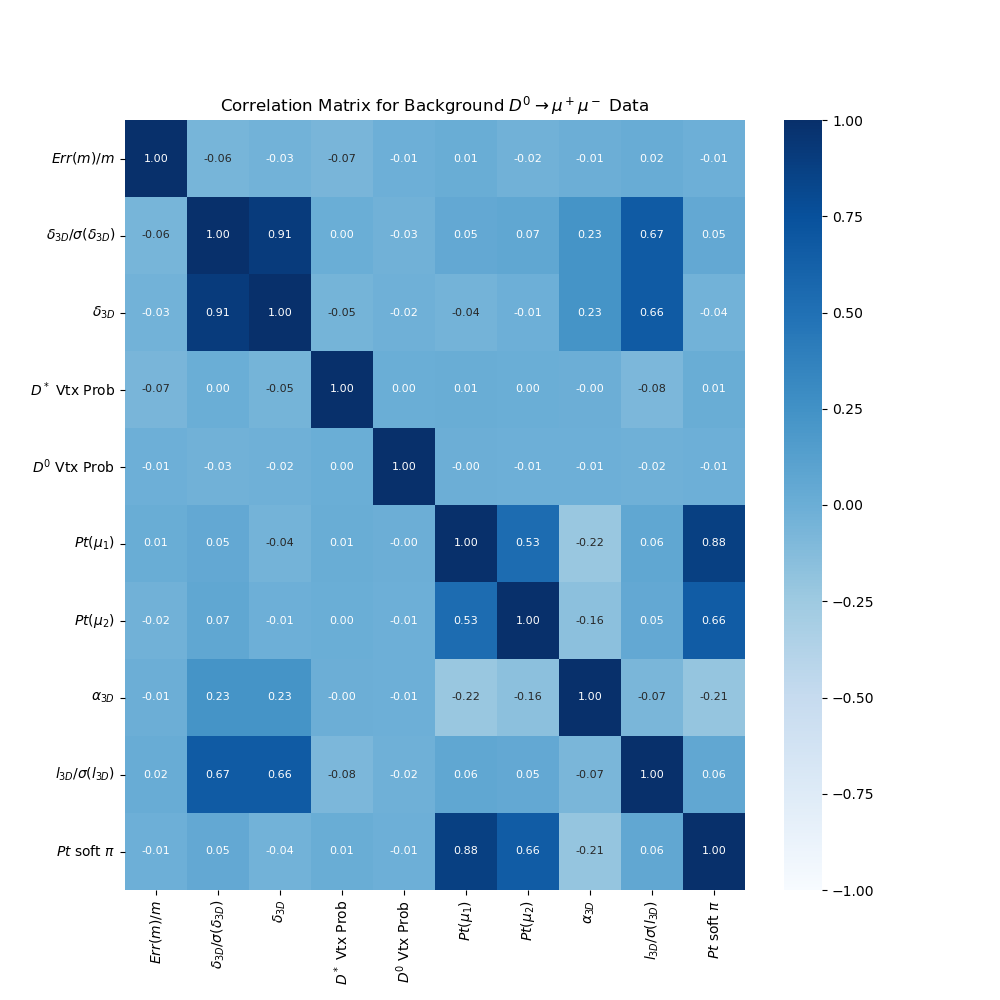
\includegraphics[width=0.45\textwidth]{figures/chapter4/mva/Correlation_data.png}
      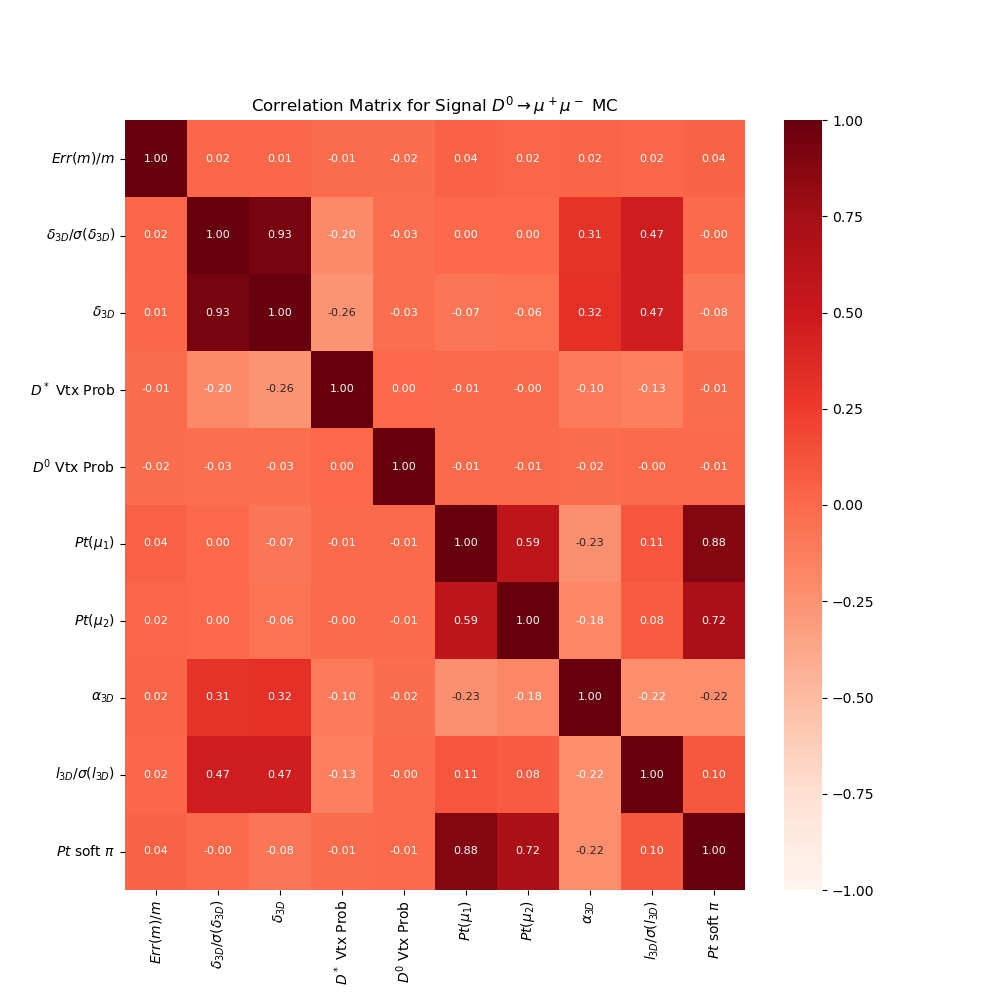
\includegraphics[width=0.45\textwidth]{figures/chapter4/mva/Correlation_dmm.png}\\
    \end{center}
    \caption{
      Correlation matrix over the MVA training variables for training background events generated from data (left) and training signal events generated from MC (right)
    }
    \label{fig:mva_correlation_matrix_for_training_variables}
\end{figure}

The correlation matrix for both the signal and background can be seen in figure \ref{fig:mva_correlation_matrix}. Importantly, there are some positive correlation between features and there are no two strong anti-correlated features, meaning we expect stability in learning due to feature redundancy and simpler interactions, yet expect good model generalization. 

Due to the relatively small amount of data avilable, the data is split into 5 groups and 5 seperate models are training, each using a different data group as testing data sets and the remaining 4 as training datasets. This ensures the models have been exposed on the entire dataset while not overfitting on any particular events. Once the models have been trained, the event number (which is independent of the contents of the event), is used to decide which model to use for classification of that event. 

It is important that the classification parameter is not correlated with any variables used later in the analysis for fitting (namely $\delta m$ and the dimuon mass) so as to not skew the fit. Due to this, the kinematic variable given to the model are restricted to $p_T$ and vertex parameters, so that it is not possible to reconstruct masses. To check that the correlations don't exist, a correlation matrix between the classification parameter, $\delta m$, and the dimuon mass is created and shown in figure \ref{fig:mva_correlation_matrix_for_fit_variables}. As expected, there is no correlation.


\begin{figure}[htp]
    \begin{center}
      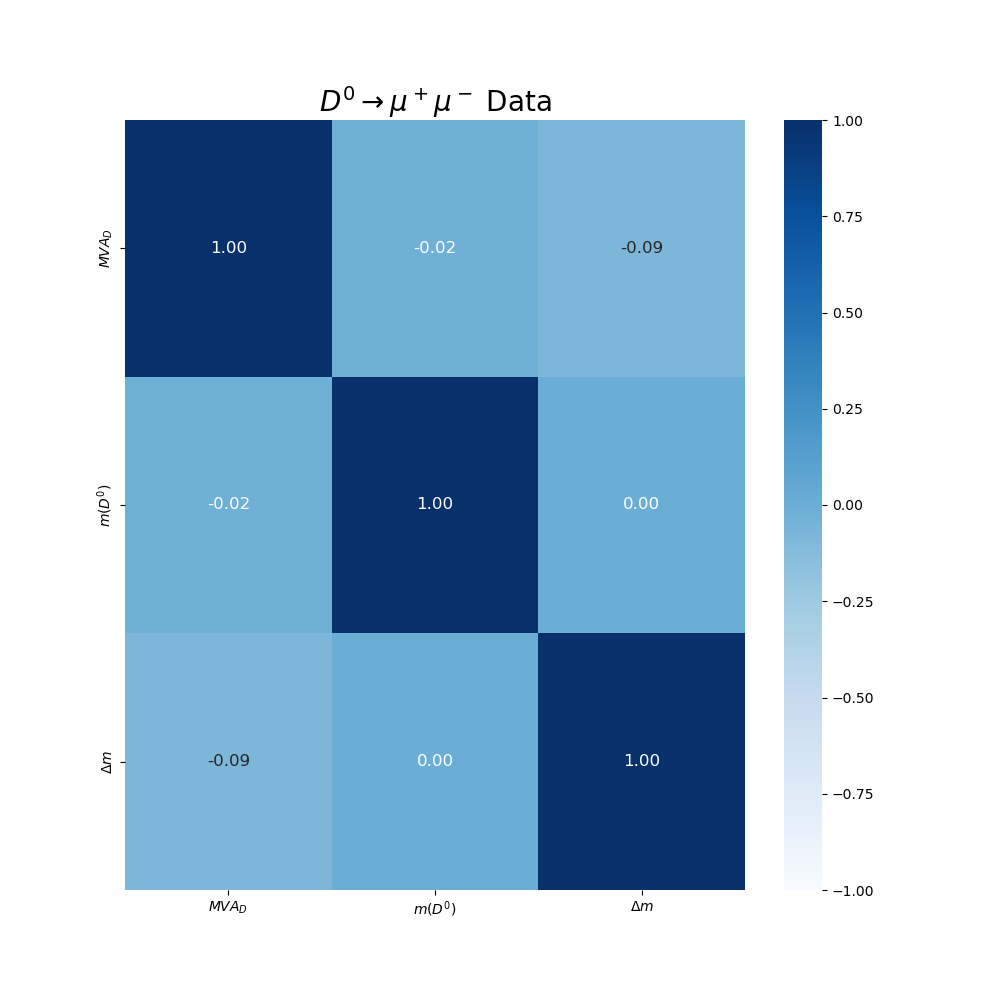
\includegraphics[width=0.45\textwidth]{figures/chapter4/mva/Correlation_data_obs.png}
      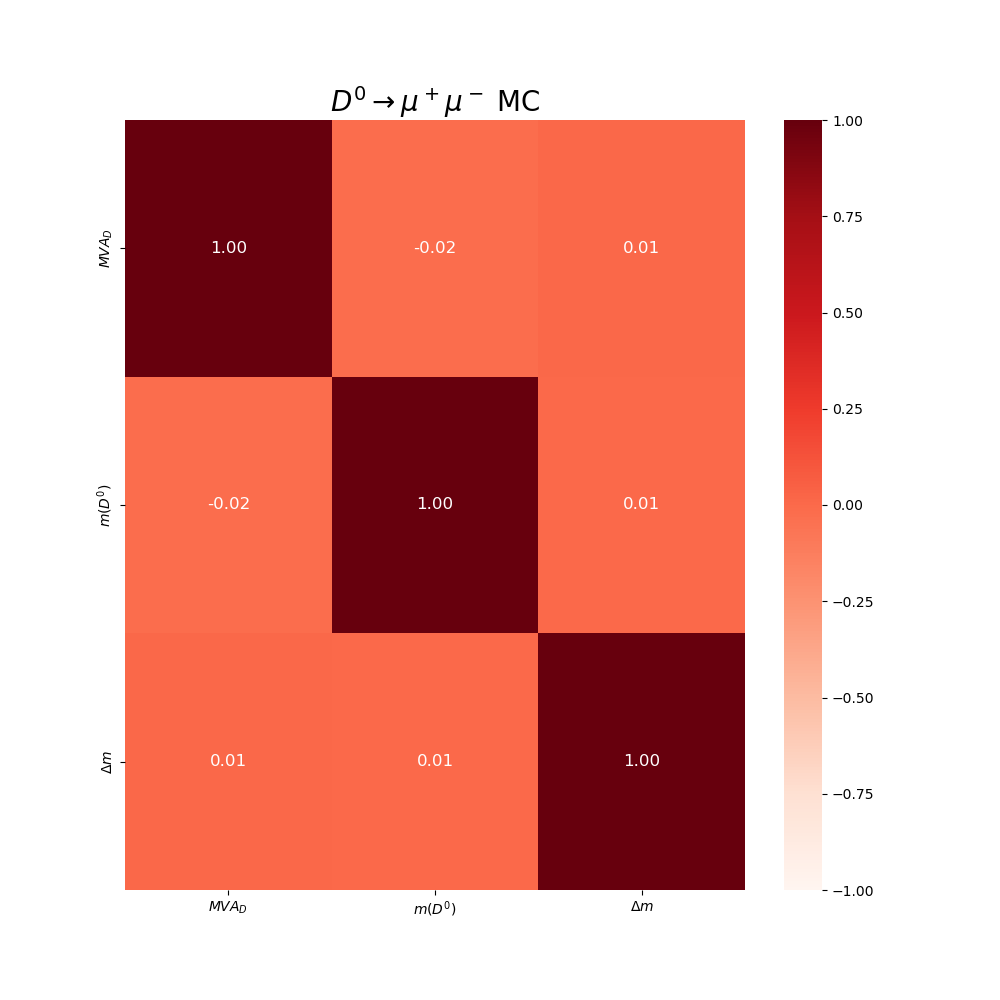
\includegraphics[width=0.45\textwidth]{figures/chapter4/mva/Correlation_dmm_obs.png}\\
    \end{center}
    \caption{
      Correlation matrix comparing the MVA classification parameter to $\delta m$ and the dimuon mass. Shown left is the training background events generated from data and shown right is the training signal events generated from MC.
    }
    \label{fig:mva_correlation_matrix_for_fit_variables}
\end{figure}

It is also important to note that the classifier is being trained and tested on simulated signal samples, yet for the analysis the efficiency of the classifier on real data is needed. Due to mismodeling effect in the simulation, the simulation efficiency is not necessarily the same as the data efficiency. Getting the efficiency is difficult to measure directly since the expected branching fraction of $D^0 \to \mu^+ \mu^-$ is so low that we do not have a reliable data sample for the signal. Instead, the efficiency is derived from the $D^0 \to \pi^+ \pi^-$ decay using the zero bias dataset and the $D^0 \to \pi^+ \pi^-$ monte-carlo simulation samples. Since the $D^0 \to \pi^+ \pi^-$ decay behaves similarly to the $D^0 \to \mu^+ \mu^-$ decay in terms of reconstruction/vertex parameters and the MVA classifier is independent of $\delta m$ and dimuon mass in both cases, the efficiency derived from $D^0 \to \pi^+ \pi^-$ is similar to the efficiency of $D^0 \to \mu^+ \mu^-$. Therefore, the same classifier with the same cut is used on both the normalization channel and the signal channel, causing the efficiencies to cancel in the branching fraction equation. TODO: link equation. We calculate the efficiency in data on the $D^0 \to \pi^+ \pi^-$ decay by performing the UML fit outlined in section TODO: (insert section link) on different $\text{MVA}_D$ cut values and comparing to the \texttt{ZeroBias} dataset. In simulated data, we are able to directly tag the signal events that were created from the simulation, so calculating the efficiency is trivial. A list of efficency values at specific $\text{MVA}_D$ cuts can be found in table \ref{tab:mva_cut_efficiencies} and a graphical representation over a more diverse $\text{MVA}_D$ cut range can be found in \ref{fig:mva_cut_efficiencies}.

\begin{table}[htbp]
    \centering
    \begin{tabular}{|l|c|c|c|}
    \hline
    $\text{MVA}_D$ cut value & \textbf{0.74} & \textbf{0.76} & \textbf{0.78} \\
    \hline
    $D^0 \to \pi^+ \pi^-$ Data Efficiency (from Zero Bias) & $0.722 \pm 0.088$ & $0.707 \pm 0.087$ & $0.681 \pm 0.086$ \\
    $D^0 \to \pi^+ \pi^-$ MC Efficiency & 0.817 & 0.801 & 0.783 \\
    $D^0 \to \mu^+ \mu^-$ MC Efficiency & 0.824 & 0.809 & 0.792 \\
    $D^0 \to \mu^+\nu_\mu\mu^-\bar{\nu}_\mu$ MC Efficiency & 0.806 & - & - \\
    \hline
    \end{tabular}
    \caption{Summary of $\text{MVA}_D$ cut efficiency at various cut values on various samples used throughout the analysis.}
    \label{tab:mva_cut_efficiencies}
\end{table}

\begin{figure}[htp]
    \begin{center}
      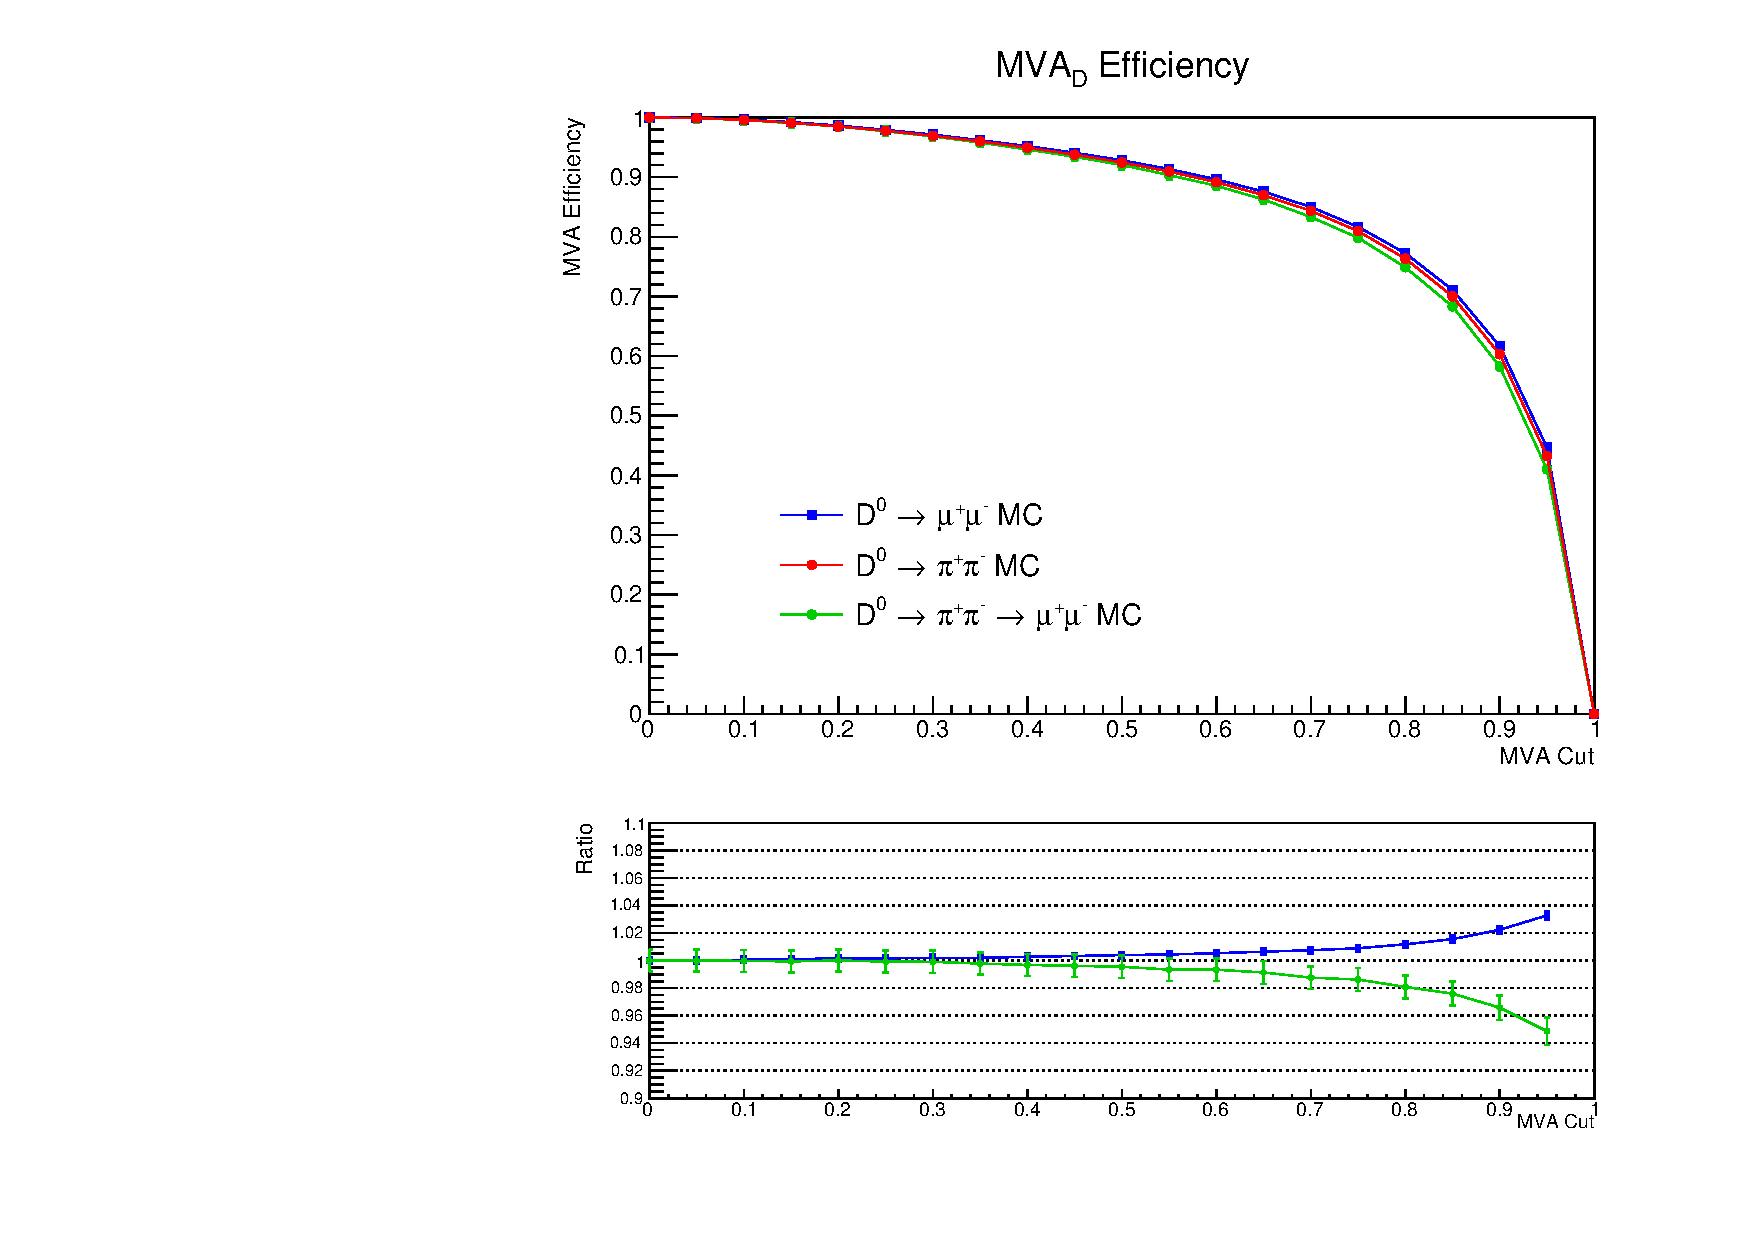
\includegraphics[width=0.5\textwidth]{figures/chapter4/mva/mva_efficiency.pdf}
    \end{center}
    \caption{
      A graphical summary of $\text{MVA}_D$ cut efficiency at various diverse cut values on various samples used throughout the analysis.
    }
    \label{fig:mva_cut_efficiencies}
\end{figure}

As can be seen in table \ref{tab:mva_cut_efficiencies} as well as figure \ref{fig:mva_cut_efficiencies}, while the efficiency values are, as expected, extremely close in the MC samples, there is still a small difference between the three decay channels. To account for this small difference, we calculate a corrective efficiency factor, derived from Monte Carlo. We name this corrective factor $\text{MVA}_{D, cor}$ and define it as
\begin{equation}
    \begin{split}
    \text{MVA}_{D,\text{cor}\;(D^0 \to \mu^+ \mu^-)} &= 
    \frac{\epsilon_{D^0 \to \mu^+ \mu^-\; \text{ (simulation)}}}
         {\epsilon_{D^0 \to \pi^+ \pi^-\; \text{ (simulation)}}} \\
    \text{MVA}_{D,\text{cor}\;(D^0 \to \pi^+ \pi^- \to \mu^+ \nu_\mu \mu^- \nu_\mu)} &= 
    \frac{\epsilon_{D^0 \to \pi^+ \pi^- \to \mu^+ \nu_\mu \mu^- \nu_\mu\; \text{ (simulation)}}}
         {\epsilon_{D^0 \to \pi^+ \pi^-\; \text{ (simulation)}}}
    \end{split}
\end{equation}
From these definitions, one can extrapolate to data due to the proximity of the efficiency values, meaning
\begin{equation}
    \begin{split}
    \epsilon_{D^0 \to \mu^+ \mu^-} \text{ (data)} &= 
    \epsilon_{D^0 \to \pi^+ \pi^-} \text{ (data)} 
    \times \text{MVA}_{D,\text{cor}\;(D^0 \to \mu^+ \mu^-)} \\
    \epsilon_{D^0 \to \pi^+ \pi^- \to \mu^+ \nu_\mu \mu^- \nu_\mu} \text{ (data)} &= 
    \epsilon_{D^0 \to \pi^+ \pi^-} \text{ (data)} 
    \times \text{MVA}_{D,\text{cor}\;(D^0 \to \pi^+ \pi^- \to \mu^+ \nu_\mu \mu^- \nu_\mu)}
    \end{split}
\end{equation}
Lastly, a very conservative systematic error is assigned to the $\text{MVA}_{D, cor}$ factors of $|1-\text{MVA}_{D, cor}|$. Therefore, we get
\begin{equation}
\begin{split}
    \text{MVA}_{D,\text{cor}\;(D^0 \to \mu^+ \mu^-)} &= 1.009\;\pm\;0.012 \; \text{(stat)}\;\pm\;0.009 \; \text{(sys)} \\
    \text{MVA}_{D,\text{cor}\;(D^0 \to \pi^+ \pi^- \to \mu^+ \nu_\mu \mu^- \nu_\mu)} &= 0.987\;\pm\;0.020 \; \text{(stat)}\;\pm\;0.013 \; \text{(sys)}
\end{split}
\end{equation}
    
\section{Unbinned Maximum Likelihood Fits}

Now that we have given accurate descriptions of the datasets and selection processes used in this analysis, we are now ready to extract the two main values needed for this analysis, the number of $D^0 \to \pi^+ \pi^-$ events, denoted $N_{D^0 \to \pi^+ \pi^-}$, the number of $D^0 \to \mu^+ \mu^-$ events, denoted $N_{D^0 \to \mu^+ \mu^-}$.

In order to do this, we perform two unbinned maximum likelihood (UML) fits on the events in our data that passes the preselection, baseline selection, and MVA selection processes. Maximum likelihood (ML) fits are statistical methods used to estimated parameters of a model given observed data. A ML fit is a UML fit when the data is not binned into a histogram, but rather the exact data values are used. UML fits define a model $f(\vec{x}; \theta, \theta_N$, which is a PDF over some set of observed variables, $\vec{x}$ and some model parameters $\theta$ and $\vec{\theta}_N$. The goal of a UML fit is to extract a model parameter $\theta$ given some observed data $\vec{x}_1, \vec{x}_2,...,\vec{x}_N$. $\vec{\theta}_N$ are considered nuisance parameters and are important to defining the model, but are not parameters of interest to the analysis. Once a model has been defined, a likelihood is defined as
\begin{equation}
    \mathcal{L}(\theta, \vec{\theta}_N) = \prod^N_{i=1} f(\vec{x}_i; \theta, \vec{\theta}_N)
\end{equation}
In this formulation, the UML fit can be represented as finding $\hat{\theta} \hat{\vec{\theta}_N}= \text{argmax}_{\theta, \vec{\theta}_N} \mathcal{L}(\theta, \vec{\theta}_N)$\footnote{In practice, this isn't quite true. Often in applications with lots of nuisance parameters, UML fits operate using profile likelihoods. However, the point of this discussion is merely an overview of UML and the complexities will be ignored.}. 

In our analysis, $\theta$ is the true number of signal events (in the normalization channel this is $N_{D^0 \to \pi^+ \pi^-}$ and in our signal channel this is $N_{D^0 \to \mu^+ \mu^-}$), $\vec{x}$ is the $\delta m$ and $m(D^0)$ of our data, and $\vec{\theta}_N$ are the variance parameters needed to construct the signal and background PDFs. A more precise discussion of this construction follows in the sections below. 

\subsection{Normalization Channel Fit}



\subsubsection{Signal Model}

\subsubsection{Background Model}

\subsubsection{Fit Results}
